\section{The Rotation Poset} 

Given the one-one correspondence between the minimal differences of $P(\mathcal{M})$ and the rotations of $\mathcal{M}$, we can finally define the long awaited representation $\Pi(\mathcal{M})$ of $\mathcal{M}$ based on rotations.

\begin{figure}[ht]
  \centering
  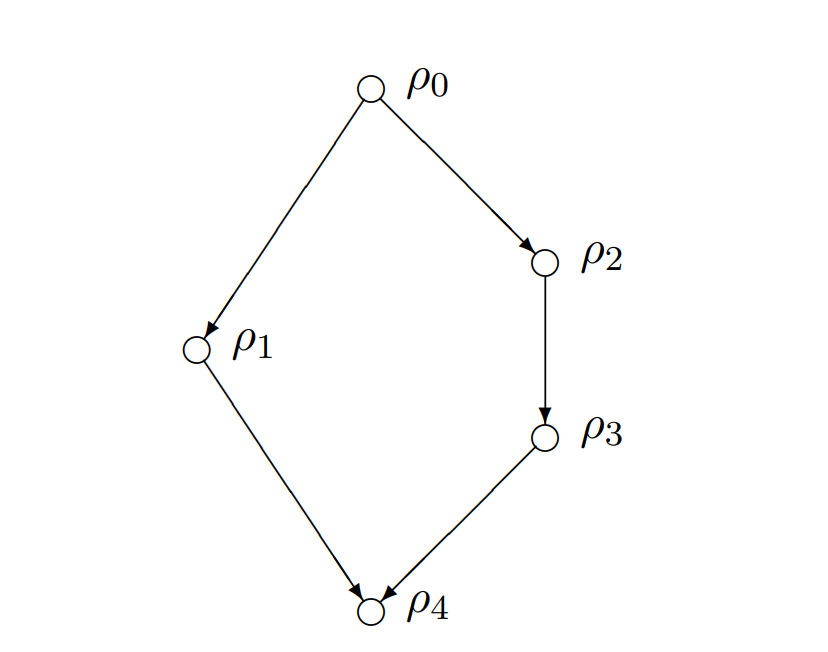
\includegraphics[width=0.4\textwidth]{IMAGES_FIGS/FIG_2_8.png}
  \caption{The rotation poset for $\mathcal{M}$}
  \label{FIG_3_10}
\end{figure}

The rotation poset of $\mathcal{M}$, denoted $\Pi(\mathcal{M})$, is the partial or der on the rotations of $\mathcal{M}$ defined by replacing each minimal difference $d(\rho)$ in the partial order $D(\mathcal{M})$ by the rotation $\rho$. The precedence relation on $\Pi(\mathcal{M})$ corresponds exactly to that on $D(\mathcal{M}): \rho^{\prime}$ precedes $\rho$ in $\Pi(\mathcal{M})$ if and only if $d\left(\rho^{\prime}\right)$ precedes $d(\rho)$ in $D(\mathcal{M})$. Note that $\Pi(\mathcal{M})$ is isomorphic to the partial order $I(\mathcal{M})$ after the removal of $M_0$ from $I(\mathcal{M})$.

\begin{theo}
    \begin{itemize}
        \item There is a one-one correspondence between the closed subsets of $\Pi(\mathcal{M})$ and the stable matchings of $\mathcal{M}$.
        \item $S$ is the closed set of rotations of $\Pi(\mathcal{M})$ corresponding to a stable matching $M$ if and only if $S$ is the (unique) set of rotations on every $M_0$-chain in $\mathcal{M}$ ending at $M$. Further, $M$ can be generated from $M_0$ by eliminating the rotations in their order along any of these paths, and these are the only ways to generate $M$ by rotation eliminations starting from $M_0$.
        \item If $S$ and $S^{\prime}$ are the unique sets of rotations corresponding to distinct stable matchings $M$ and $M^{\prime}$, then $M$ dominates $M^{\prime}$ if and only if $S \subset S^{\prime}$.
    \end{itemize}
\end{theo} 
